\documentclass[12pt]{article}
\usepackage[]{color}

%% maxwidth is the original width if it is less than linewidth
%% otherwise use linewidth (to make sure the graphics do not exceed the margin)
\makeatletter
\def\maxwidth{ %
	\ifdim\Gin@nat@width>\linewidth
	\linewidth
	\else
	\Gin@nat@width
	\fi
}
\makeatother

\definecolor{fgcolor}{rgb}{0.345, 0.345, 0.345}
\newcommand{\hlnum}[1]{\textcolor[rgb]{0.686,0.059,0.569}{#1}}%
\newcommand{\hlstr}[1]{\textcolor[rgb]{0.192,0.494,0.8}{#1}}%
\newcommand{\hlcom}[1]{\textcolor[rgb]{0.678,0.584,0.686}{\textit{#1}}}%
\newcommand{\hlopt}[1]{\textcolor[rgb]{0,0,0}{#1}}%
\newcommand{\hlstd}[1]{\textcolor[rgb]{0.345,0.345,0.345}{#1}}%
\newcommand{\hlkwa}[1]{\textcolor[rgb]{0.161,0.373,0.58}{\textbf{#1}}}%
\newcommand{\hlkwb}[1]{\textcolor[rgb]{0.69,0.353,0.396}{#1}}%
\newcommand{\hlkwc}[1]{\textcolor[rgb]{0.333,0.667,0.333}{#1}}%
\newcommand{\hlkwd}[1]{\textcolor[rgb]{0.7te37,0.353,0.396}{\textbf{#1}}}%

%\usepackage{framed}
%\makeatletter
%\newenvironment{kframe}{%
%	\def\at@end@of@kframe{}%
%	\ifinner\ifhmode%
%	\def\at@end@of@kframe{\end{minipage}}%
%\begin{minipage}{\columnwidth}%
%	\fi\fi%
%	\def\FrameCommand##1{\hskip\@totalleftmargin \hskip-\fboxsep
%		\colorbox{shadecolor}{##1}\hskip-\fboxsep
%		% There is no \\@totalrightmargin, so:
%		\hskip-\linewidth \hskip-\@totalleftmargin \hskip\columnwidth}%
%	\MakeFramed {\advance\hsize-\width
%		\@totalleftmargin\z@ \linewidth\hsize
%		\@setminipage}}%
%{\par\unskip\endMakeFramed%
%	\at@end@of@kframe}
%\makeatother

\definecolor{shadecolor}{rgb}{.97, .97, .97}
\definecolor{messagecolor}{rgb}{0, 0, 0}
\definecolor{warningcolor}{rgb}{1, 0, 1}
\definecolor{errorcolor}{rgb}{1, 0, 0}
\newenvironment{knitrout}{}{} % an empty environment to be redefined in TeX

%%% FONT AND INPUT
\usepackage[T5]{fontenc}
\usepackage[utf8]{inputenc} % set input encoding (not needed with XeLaTeX)

%%% Examples of Article customizations
% These packages are optional, depending whether you want the features they provide.
% See the LaTeX Companion or other references for full information.

%%% PAGE DIMENSIONS
\usepackage{geometry} % to change the page dimensions
\geometry{letterpaper} % or letterpaper (US) or a5paper or....
\geometry{margin=1in} % for example, change the margins to 2 inches all round
% \geometry{landscape} % set up the page for landscape
%   read geometry.pdf for detailed page layout information

\usepackage{graphicx} % support the \includegraphics command and options

% \usepackage[parfill]{parskip} % Activate to begin paragraphs with an empty line rather than an indent

%%% PACKAGES
\usepackage{booktabs} % for much better looking tables
\usepackage{array} % for better arrays (eg matrices) in maths
\usepackage{paralist} % very flexible & customisable lists (eg. enumerate/itemize, etc.)
\usepackage{verbatim} % adds environment for commenting out blocks of text & for better verbatim
\usepackage{subcaption} % make it possible to include more than one captioned figure/table in a single float
\usepackage{float}
\usepackage{setspace}
\usepackage{amsmath,newtxtext,newtxmath}
\usepackage{url}
\usepackage{multirow}
\usepackage{listings}
\usepackage{dcolumn}
%\usepackage[nolists]{endfloat}
\usepackage{bbm}
\usepackage{pdflscape}
\usepackage{pdfpages}
\usepackage{xr} % to use \ref with labels from the main text
\externaldocument{'200129 - AJPS RnR Draft 1'}
\usepackage{tikz} 
\usetikzlibrary{arrows,decorations.pathmorphing,decorations.pathreplacing,backgrounds,fit,positioning,shapes.symbols,chains}

%%% HEADERS & FOOTERS
\usepackage{fancyhdr} % This should be set AFTER setting up the page geometry
\pagestyle{fancy} % options: empty , plain , fancy
\renewcommand{\headrulewidth}{0pt} % customise the layout...
\lhead{}\chead{}\rhead{}
\lfoot{}\cfoot{\thepage}\rfoot{}

%%% CITATION AND BIBLIOGRAPHY

\usepackage[authordate,backend=bibtex8,natbib,sorting=nyt,sortcites,isbn=false,doi=false]{biblatex-chicago}
%\usepackage{natbib}
%\bibliographystyle{apsr}
\bibliography{Literature/library_syp}

% fix problem with \citeyear and \citeyearpar not being highlighted
\DeclareCiteCommand{\citeyear}
	{}
	{\bibhyperref{\printdate}}
	{\multicitedelim}
	{}

\DeclareCiteCommand{\citeyearpar}
	{}
	{\mkbibparens{\bibhyperref{\printdate}}}
	{\multicitedelim}
	{}
% possessive cite with \citepos
\newcommand\citepos[1]{\citeauthor{#1}'s\ (\citeyear{#1})}


\usepackage{hyperref}
\hypersetup{
	colorlinks=true,
	linkcolor=blue,
	filecolor=magenta,      
	urlcolor=cyan,
}

%%% SECTION TITLE APPEARANCE
\usepackage{sectsty}
%\allsectionsfont{\sffamily\mdseries\upshape} % (See the fntguide.pdf for font help)
% (This matches ConTeXt defaults)

%%% ToC (table of contents) APPEARANCE
\usepackage[nottoc,notlof,notlot]{tocbibind} % Put the bibliography in the ToC
\usepackage[titles,subfigure]{tocloft} % Alter the style of the Table of Contents
\renewcommand{\cftsecfont}{\rmfamily\mdseries\upshape}
\renewcommand{\cftsecpagefont}{\rmfamily\mdseries\upshape} % No bold!

%%% Some commands
\newcommand{\reg}{\texttt{regress} }
\newcommand{\1}{\mathbbm{1}}

\renewcommand\r{\right}
\renewcommand\l{\left}
\newcommand\E{\mathbbm{E}}
\newcommand\V{\mathbbm{V}}
\newcommand\Var{\mathbbm{V}}
\newcommand\avar{{\rm Avar}}
\newcommand\dist{\buildrel\rm d\over\sim}
\newcommand\iid{\stackrel{\rm i.i.d.}{\sim}}
\newcommand\ind{\stackrel{\rm indep.}{\sim}}
\newcommand\cov{{\rm Cov}}
\newcommand{\R}{\textbf{R} }
\newcommand{\Rcmd}[1]{{\large \texttt{#1}}}
\newcommand\indep{\protect\mathpalette{\protect\independenT}{\perp}}
\def\independenT#1#2{\mathrel{\rlap{$#1#2$}\mkern2mu{#1#2}}}
\DeclareMathOperator{\sgn}{sgn}
\DeclareMathOperator*{\argmin}{argmin}

\newcommand\Sum{\sum^N_{i=1}}
\newcommand\Prod{\prod^N_{i=1}}
\newcommand{\pderiv}[1]{\frac{\partial}{\partial #1}}
\newcommand{\B}[1]{\boldsymbol{#1}}
\newcommand{\logit}{\text{logit}}

%%% texcount
% Run texcount on tex-file and write results to a sum-file
\immediate\write18{texcount  \jobname.tex -out=\jobname.sum -incbib -relaxed}
% Define macro \wordcount for including the counts
\newcommand\wordcount{\verbatiminput{\jobname.sum}}


%opening
\title{Tea Leaf Elections: \\
	Inferring Purpose for Authoritarian Elections from Post-election Responses to Defeats \\
	\vspace{2ex}
	Online Appendix}
%\author{Minh Trinh}
\date{July 31, 2019}

\begin{document}
	
%TC:ignore 

\maketitle
\thispagestyle{empty}

%TC:endignore 

\doublespacing

\newpage
\pagenumbering{arabic}

\tableofcontents
\newpage

\appendix

\section{Digit tests showing no evidence of high-level manipulation}
\label{app:benford}
To verify that the CPV does not engage in overt \textit{ex-post} manipulation of vote results at the high level (for example by changing the vote tallies), I conduct several digit tests on official results from the 2011 and 2016 elections. 

Digit-based tests have been used widely in the election forensics literature to detect evidence of fraud both in American \citep{Mebane2006} and Comparative Politics \citep{Mebane2009, Beber2012}. Many of these tests are based on Benford's Law, which states that digits in naturally occurring numbers follow certain patterns, and that human interventions in the data generation process can lead to violation of these patterns. Because many numbers produced in an elections such as vote counts or turnout figures are naturally occurring numbers, they can be tested against the patterns to detect suggestive evidence of human tampering \citep{Mebane2006}. Under the null hypothesis, Benford's Law suggests that the probability that the first $m$ digits of a number follow a particular sequence is given by:
\begin{align*}
P(D_1=d_1, D_2=d_2, \dots, D_m=d_m) &= \log_{10}\l(1 + \l( \sum_{j=1}^{m}10^{m-j}d_j\r)\r)
\end{align*}
where $D_i$ represents the $i$th significant digit, and $d_i$ is a particular realization of that digit. From this, it is possible to calculate the Benford Distribution for the First Digit:
\begin{align*}
P(D_1=d_1) = \log_{10}\l(1 + \frac{1}{d_1}\r)
\end{align*}
as well as the Benford Distribution for the Second Digit:
\begin{align*}
P(D_2=d_2) = \sum_{j=1}^{9}\log_{10}\l(1 + \frac{1}{10j + d_2}\r)
\end{align*}
and for the Third Digit:
\begin{align*}
P(D_3=d_3) = \sum_{k=1}^{9}\sum_{j=0}^{9}\log_{10}\l(1 + \frac{1}{100k + 10j + d_3}\r)
\end{align*}
and so on. Note that as $i$ increases, the distribution converges quickly to uniform.

To test whether the Vietnamese regime has tampered with the final, aggregated results from VNA elections, I conduct digit tests on numbers from the publicly released results following the 2011 and 2016 elections. The hypothesis is that if the CPV has tampered with the results, at least some digits in these numbers would be found to violate Benford's Law. 

The format of the public release change from one election to another. Specifically, in 2011 the official release includes district-level information such as the number of eligible voters, turnout, the number of invalid votes, but lists only the vote shares of winning candidates. In 2016, however, the official release lists out the vote counts and vote shares of every candidate, but omist district-level information. As a result, I choose different sets of numbers to conduct digit tests on: turnout and number of invalid votes for the 2011 election, and candidate vote counts for the 2016 election. Unlike vote shares, which \citet{MaleskySchuler2011} use, these numbers are not bounded above and beyond, are not subjected to rounding, and span multiple orders of magnitude, which are requirements for Benford-like number distributions \citep{Hill1995, Mebane2006, Berger2015}.

Figure \ref{fig:Benford} shows the results, in the form of histograms for the empirical distribution of digit values for each of the first three significant digits of each measure, overlaid with the expected Benford distribution and a 95\% confidence interval. As \citet{Mebane2006} notes, the first digit of vote counts and turnout figures do \textit{not} follow Benford's Law, as they are often constrained by district sizes. No such constraint applies for the first digits of invalid votes, as well as every other digit of all three measures, and so we expect the empirical and expected distributions to be close in all but the upper-left and lower-left graphs in Figure \ref{fig:Benford}. This indeed turns out to be the case except for some few exceptions. Note further that the confidence intervals have not been adjusted for multiple testing, and if this is done all of the bars in Figure \ref{fig:Benford} would fall within these intervals. Finally, I also conduct chi-squared and Kolmogorov-Smirnov tests, and found no significant results even before correcting for multiple testing. Altogether, these tests fail to reject the null hypothesis of no manipulation, at least at the highest levels.

\begin{figure}[!htbp]
	\centering
	
\includegraphics[height=.85\textheight]{figure/190716_digit_test.png}
	\caption[Digit Test of Election Results]{Empirical distribution (as bars) and expected distribution under Benford's Law (as dashed lines) of first, second, and third digits of district-level voter turnouts in the 2011 election, district-level invalid vote counts in the 2011 election, and district-level vote counts by candidate in the 2016 election. Shaded regions denote 95\% confidence intervals around the expected distributions. The first digits of 2011 Turnout and 2016 Vote counts (highlighted with \textsf{*}) are expected to violate Benford's Law even without tampering.}
	\label{fig:Benford}
\end{figure}

\clearpage

\section{Effect of 2015 State Budget Law}

In 2015, the Vietnamese government issued a revised Law on the State Budget (hereafter 2015 State Budget Law), which became effective from the 2017 fiscal year. Among other changes, the revised law reiterated the centrality of the central government budget in fiscal governance i.e. fiscal recentralization. Practically, the 2015 State Budget Law led to major adjustments to provincial budgets, particularly through changes in the proportions of the shared revenue that provinces have to remit back to the central government (recall that the revenue generated into each province can be divided into three categories: revenues that belong to the province exclusively, revenues that belong to the central government exclusively, and revenues that must be shared between the provincial and the central government according to a fixed ratio). \autoref{tab:2015_budget_law_changes} lists out provinces that were impacted by these adjustments, along with the proportions they get to keep from the shared revenues before and after the adjustments.

\begin{table}[!htp]
	\centering
		\begin{tabular}{@{}lccll@{}}
			\toprule
			&
			\multicolumn{1}{c}{\begin{tabular}[c]{@{}c@{}}2011-2016\\ proportions\end{tabular}} &
			\multicolumn{1}{c}{\begin{tabular}[c]{@{}c@{}}2017-2020\\ proportions\end{tabular}} &
			\multicolumn{1}{c}{\begin{tabular}[c]{@{}c@{}}Close \\ defeat(s)?\end{tabular}} &
			\multicolumn{1}{c}{\begin{tabular}[c]{@{}c@{}}Close \\ victor()ies)?\end{tabular}} \\ \midrule
			Ho Chi Minh City & .23 & .18 & \multicolumn{1}{c}{Y} & \multicolumn{1}{c}{Y} \\
			Binh Duong       & .40 & .36 & \multicolumn{1}{c}{}  & \multicolumn{1}{c}{Y} \\
			Ha Noi           & .42 & .35 & \multicolumn{1}{c}{Y} & \multicolumn{1}{c}{Y} \\
			Ba Ria-Vung Tau  & .44 & .64 &                       &                       \\
			Dong Nai         & .51 & .47 &                       &                       \\
			Vinh Phuc        & .60 & .53 &                       &                       \\
			Quang Ngai       & .61 & .88 &                       &                       \\
			Quang Ninh       & .70 & .65 &                       &                       \\
			Khanh Hoa        & .77 & .72 &                       &                       \\
			Da Nang          & .85 & .68 &                       &                       \\
			Hai Phong        & .88 & .78 &                       &                       \\
			Bac Ninh         & .93 & .83 &                       &                       \\
			Quang Nam        & 1   & .90 &                       &                       \\
			Hung Yen         & 1   & .93 &                       &                       \\
			Hai Duong        & 1   & .98 &                       &                       \\ \bottomrule
		\end{tabular}
	\caption{Table showing changes to the proportions that individual provinces get to keep out of revenue sources designated as ``shared revenues.'' Sources: adapted from \autocite{BaoViet} with updated data from Ministry of Finance.}
	\label{tab:2015_budget_law_changes} 
\end{table}

Because the changes to the proportions became effective in 2017, the same post-election year that budgetary responses to localized defeats are expected to take place, they could potentially confound the results. Specifically, because the changes mostly result in more productive provinces having to surrender a larger share of their revenues to the central government (with the exception of oil-producing Ba Ria-Vung Tau and Quang Ngai), and because \autoref{tab:balance} in the paper indicates these provinces are more likely to experience central candidate defeats (this difference is not statistically significant, nonetheless), the confounding may lead to an upward bias in the effect estimates.

However, the confounding does not compromise any of the main findings because there is little overlap between the provinces affected by the 2015 State Budget Law and those included in the analyses' samples. Columns 4 and 5 of \autoref{tab:2015_budget_law_changes} lists out which of the former group of provinces have encountered close central candidate defeats or victories in the 2016 election. With the exception of Ha Noi and Ho Chi Minh City, which are already excluded from analysis for other reasons, and Can Tho, which experienced no significant adjustment, Binh Duong remains the only province in the main analysis for which the confounding could manifest. Given the large size of the province's economy which makes it a likely influential outlier, prudence suggests that I exclude it from the main analysis.

With Binh Duong excluded from the sample, the main effect estimates should no longer be confounded by budgetary changes following the 2015 State Budget Law. They remain consistently positive and statistically significant, confirming that the findings are not driven by the effect of the 2015 State Budget Law. When compared with an analysis that includes it, the point estimates for the linear fixed effects models are smaller, suggesting that the risk of confounding is indeed non-trivial and the exclusion of Binh Duong indeed leads to more conservative results. Reassuringly, the sample without Binh Duong exhibits better balance, in terms of both pre-treatment covariates and pre-treatment outcomes.

\clearpage

\section{Extending main analysis to previous elections}

\subsection{Why focus on the 2016 election?}

The analysis in the main paper focus on the 2016 election to achieve the maximum inferential leverage. Compared to previous elections in 2011 and 2007\footnote{Data from elections before 2007 are not available.} the 2016 election offers significantly more valuable data in two ways. First, only in 2016 did the CPV include vote shares for defeated candidates when releasing election results. Official result releases in previous elections would only list out the names and vote shares of elected candidates, along with district-level statistics such as turnout. Although defeated candidates can still be identified by comparing the pre-election candidate list with the final results, it is impossible to determine the margin by which each of them had lost. Information about margins is important because it helps separate out central candidate defeats that were close and hence truly surprising, versus defeats that seemed too certain to be unexpected. Central candidates who lost by large margins are likely to be different from those who did only narrowly, and provinces where heavy defeats happened are also likely to be different as well. At the candidate level, heavy losers may be unpopular with both the voting public and the provincial Party apparatus. They may also be ``undesirable'' elites that the ruling party wishes to punish by forcing to contest an unwinnable election.\footnote{I thank an anonymous reviewer for suggesting this possibility.} At the province level, heavy defeats are more likely to be signal blatant acts of resistance by provincial officials, acts that could only be expected from the most defiant provinces, which are also likely to be those most financially independent of the central government. In each of these scenarios, what sets the candidates or the provinces apart -- the candidates' unpopularity or the provinces' defiance -- must be serious enough that it cannot go unnoticed. In other words, when heavy defeats happen, the central leadership is likely to already know the underlying causes. Unlike close defeats which may have surprised the CPV, heavy defeats thus bring less information content, and are less likely to elicit the same kind of response. Including these defeats in the analysis would lead to no new insights about how the regime acquires and reacts to information from elections, and in practice may lead to bias.

Specifically, bias induced by the uniqueness of heavy defeats could manifest in two different ways. Firstly, if these defeats were not surprising and thus did not induce any reaction by the regime, then an estimate of their ``treatment effect'' would likely be zero, which would then bias the average treatment effect estimate downwards. Conversely, if heavy defeats actually indicate successful attempts by provincial officials to punish undesirable elites on behalf of the regime, then estimates of the average treatment effect would be inflated by any budgetary rewards that the provinces may receive for such successes. Secondly and more importantly, if heavy defeats reflect high degree of independence by the provinces, then both the level of central transfers these provinces received in the election year, as well as the year-to-year changes over preceding years, are likely to be different. The result is the problem of dynamic causality, occurring because past central transfers are almost certainly determinants of present central candidate defeats. Because provinces with heavy defeats differ from provinces with no defeats both in the level of potential outcomes as well as the probability of receiving defeats, the difference in post-election central transfers between these sets of provinces no longer reflects a true, unbiased treatment effect of localized defeats.

The second benefit of focusing on the 2016 election is that it offers a longer pre-treatment period for the generalized synthetic control method \citep{Xu2017gsynth}. Given that budgetary data for Vietnam is only available from 2004, an analysis focused on the 2016 election and hence designating 2017 as the first post-treatment year would have 13 pre-treatment years, much closer to \citepos{Abadie2010} recommendation than the 8 pre-treatment years available for an analysis focused on the 2011 election. The longer pre-treatment period allows more data to go into the construction of the synthetic control, which in turn leads to a more inferentially valid comparison. In addition, the synthetic control constructed from thinner data is less likely to perfectly match treated observations' outcome history, and is thus less effective at tackling dynamic causality.

When the sample is dynamically balanced like in the main analysis i.e. when treated and control provinces have similar outcome values in multiple pre-treatment years, inferences using the generalized synthetic control method are unlikely to diverge from linear fixed effects models, and thus function primarily to further validate these results. When there is significant threat of dynamic causality, however, the generalized synthetic control method is the only way to mitigate this problem. Because the sample from the 2007 and 2011 elections are likely to suffer from dynamic causality, but does not have sufficient data for the generalized synthetic control method to perform optimally, the main analysis prioritizes data from the 2016 election to achieve the maximum level of internal validity.

\subsection{Responses to localized defeats in 2011 election}

Even though focusing on the 2016 election would lead to the most internally valid inferences, external validity requires that I identify whether similar increases in central transfers can also be observed following localized defeats of central candidates in previous elections. I thus attempt to extend the main analysis in this paper to the 2011 and 2007 elections, the only remaining elections for which data is available, starting with the 2011 election.

As discussed above, I anticipate several analytical challenges. For the linear fixed effects models, the inability to filter out provinces with large and unsurprising defeats leads means I have to count all provinces that experienced any central candidate defeat as ``treated.''\footnote{I also have to identify close victories using each winner's vote shares instead of their margins vis-\`{a}-vis the highest-winning loser. Specifically, I code a district as experiencing a close victory if the lowest-winning candidate's vote shares is less than 60 percent. This procedure may lead to some truly close victories not being included in the sample. For example, a candidate with a vote share of 65 percent may still win narrowly if the next candidate has secured support from 56 percent of the voters.} This is expected to result in important pre-treatment dissimilarity between treated and control provinces. Although the models' inferences are only valid for provinces with narrow central candidate victories and defeats, the 2011 treated pool also contains an unknown number of provinces with only heavy defeats. Because these provinces are not comparable to provinces with close central candidate defeats, and thus are not comparable to provinces with close central candidate victories, estimates of the treatment effect is likely to be biased. \autoref{fig:lfe_placebo_2011}, which plots estimates of the treatment effect for the 2011 election against three placebo treatment effects estimated by assuming the 2011 election has instead happened in 2008, 2009, and 2010, confirms this concern. Specifically, there are large placebo effects detected for 2009 and 2010, which should not be expected if treated and control provinces are comparable. The 2009 placebo in particular are large enough to be statistically significant at the .1 and .05 level, depending on specification. When compared to placebo effects estimated in the 2016 analysis, each placebo effect for 2011 is much larger than the corresponding effect for 2016, suggesting serious dynamic imbalance. For this reason, the main effect estimates, which are negative and indistinguishable from zero, should not be considered as reliable.

\begin{figure}[!htbp]
	\centering
	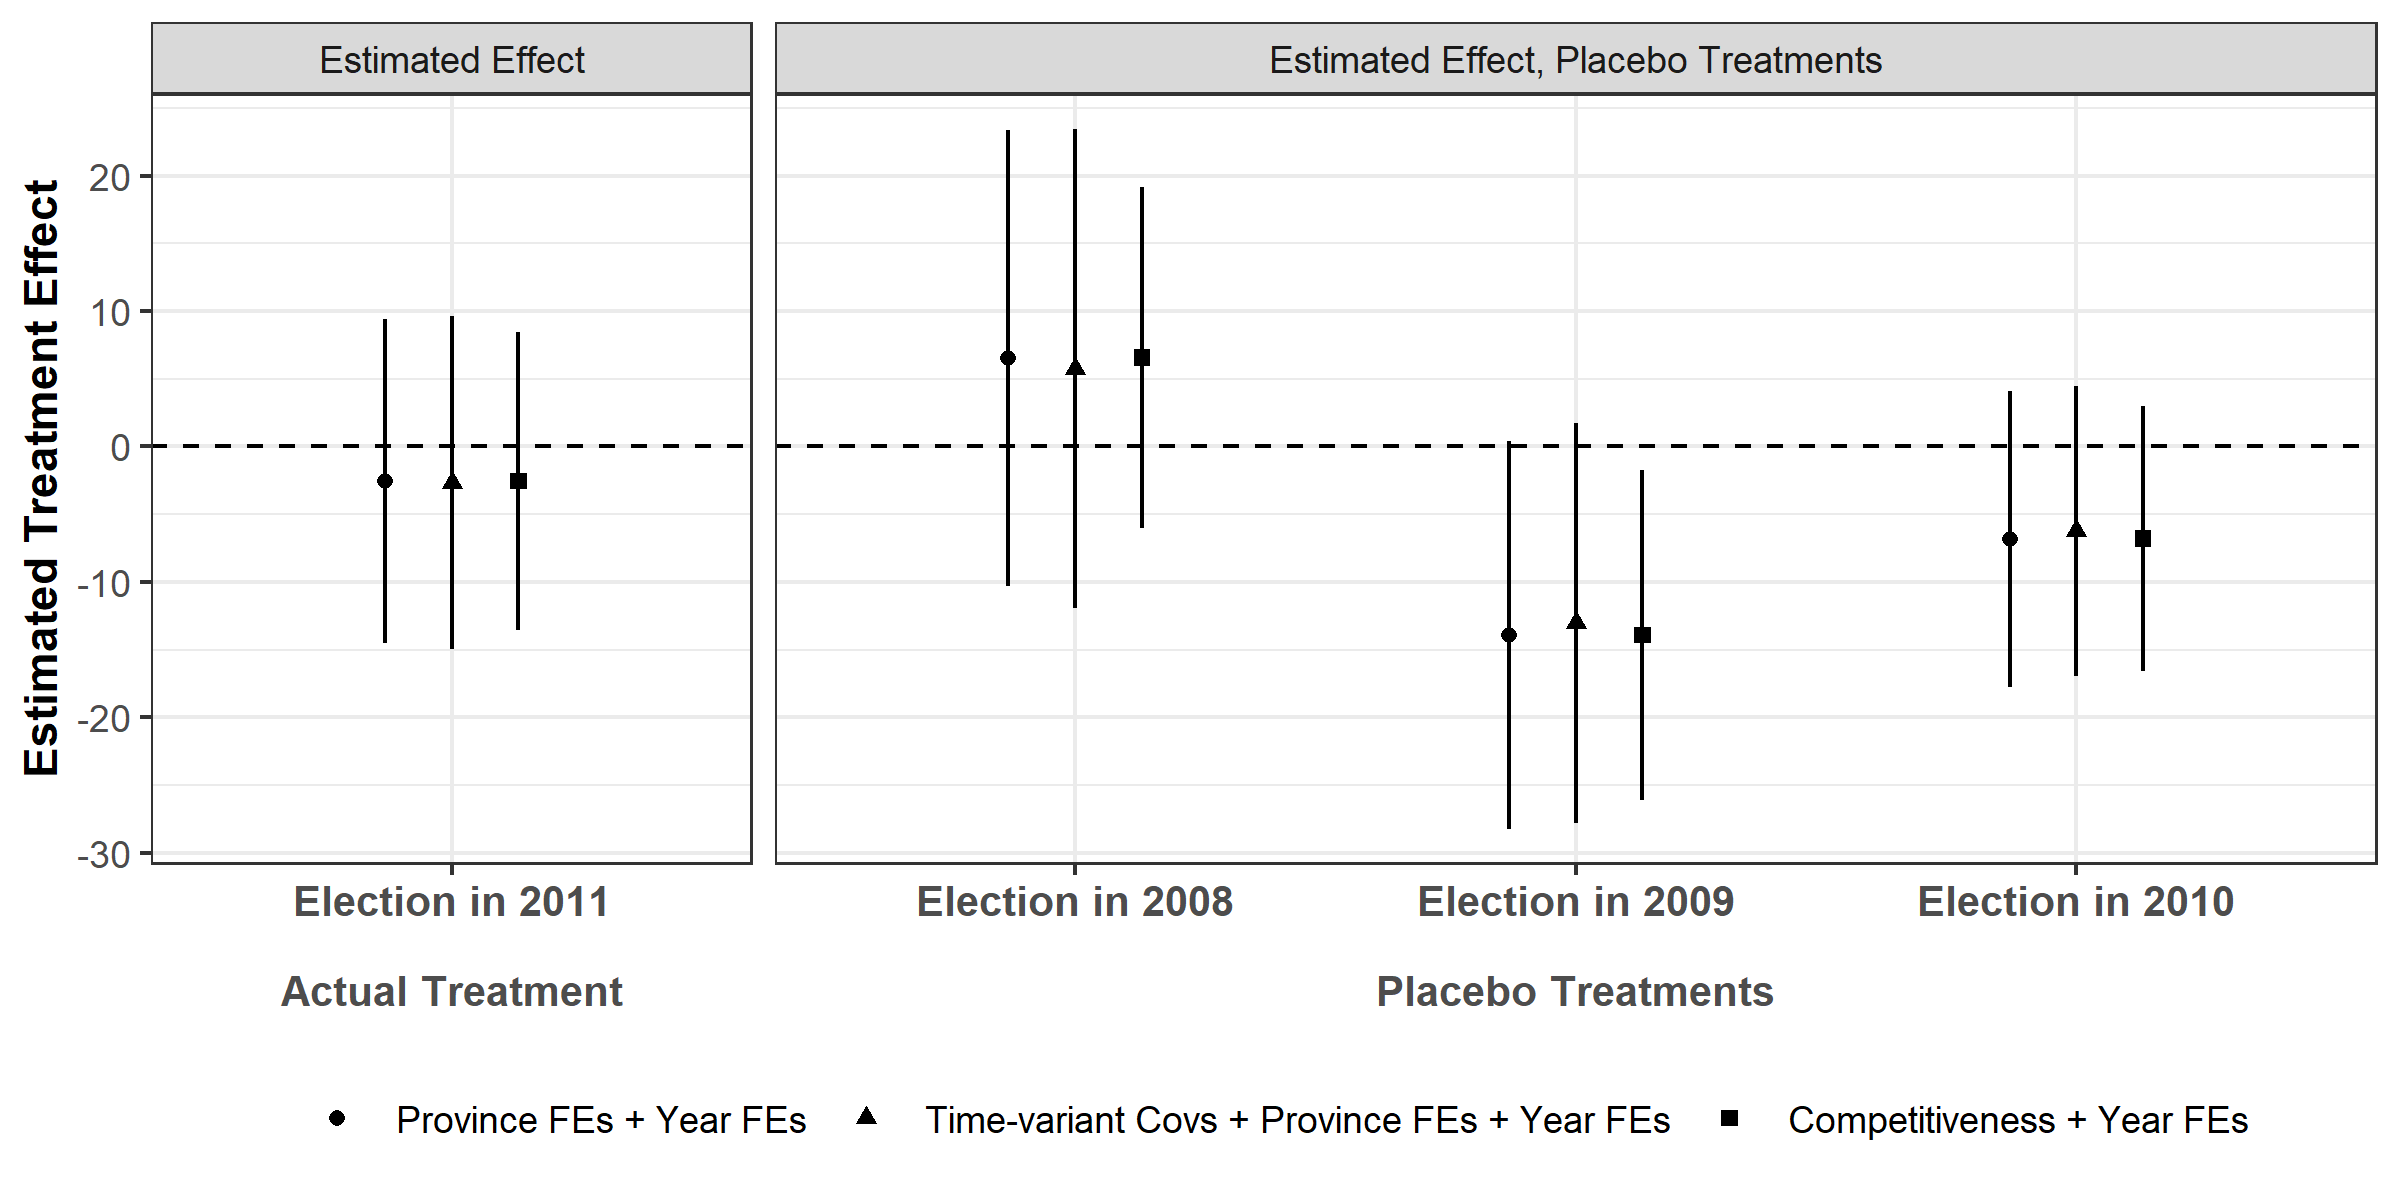
\includegraphics[width=\textwidth]{figure/200202_lfe_placebo_2011.png}
	\captionsetup{singlelinecheck=off}
	\caption[Estimated placebo linear fixed effects treatment effects for 2011]{Estimates of instantaneous treatment effects for the 2011 election using linear fixed effects models. All central candidate defeats are included in the sample. The error bars show 95\% confidence intervals.}
	\label{fig:lfe_placebo_2011}
\end{figure}

To compound the problem, the candidate-level local randomization procedure is no longer appropriate for this case. Recall that this procedure involves identifying a window of vote margin boundaries, such that central candidates who lost and won with margins within this window can be considered to have had their result assigned as-if randomly. Without vote share data from defeated candidates to calculate margins, no such boundaries can be defined. The closest alternative is an one-sided window defined by an upper boundary on winners' vote shares, such that the sample would include all central candidates who won with vote shares smaller than it. The resulting window, however, would still include all defeated central candidates, including those whose defeats are too severe to ever be considered as-if random. This undermines the logic of the regression discontinuity framework, and thus would not lead to appropriate inferences.

In light of the problem facing the linear fixed effects analysis, and the inapplicability of the local randomization approach, the generalized synthetic control method \citep{Xu2017gsynth} becomes much more important. Compared to linear fixed effects model, it is more effective at addressing dynamic causality, even when it is unable to account for unobserved time-invariant confounders \autocite{ImaiKim2019}. Given the possibility of dynamic imbalance revealed in \autoref{fig:lfe_placebo_2011}, this method seems preferable for the 2011 analysis.

\autoref{fig:synth_results_2011} shows the result from an analysis applying the generalized synthetic control method \citep{Xu2017gsynth} to data from the 2011 election. Most importantly, it shows that estimates of localized defeats' treatment effect is positive in all post-treatment years, with magnitude increasing the further away from the election year and becoming statistically significant (at the .05 level) in 2015. The method has mitigated pre-treatment differences in net transfers between treated and control provinces, as evident in the much smaller placebo treatment effects at 2009, 2010, and 2011. Because it uses data from only a short pre-treatment period, however, the generalized synthetic control in this analysis is still far from a perfect match to the treated pool. In particular, some concerns about dynamic imbalance remain, given that the difference in outcome at 2011 is still statistically significant at the .1 level. At the same time, when compared with results from the linear fixed effects, it is possible to see that the magnitude of the treatment effect increases as dynamic imbalance is reduced, suggesting that the confounding induced by dynamic causality may have led to a downward bias. In any case, the evidence from this analysis, though tentative, does suggest a positive effect i.e. an increase in central transfers to provinces that experienced localized defeats.

\begin{figure}[!h]
	\centering
	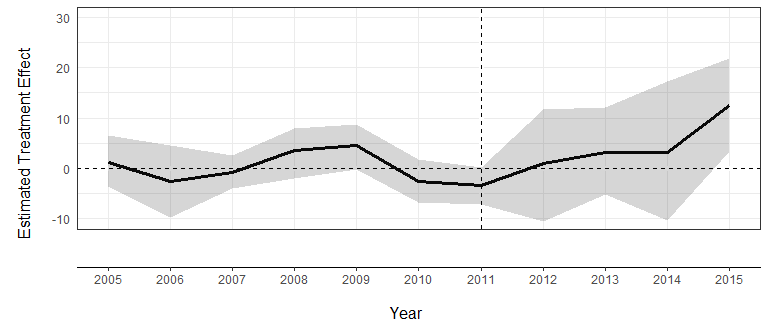
\includegraphics[width=\textwidth]{figure/200202_synth_results_2011.png}
	\captionsetup{singlelinecheck=off}
	\caption[Estimated synthetic control treatment effects for 2011]{Estimates of treatment effects for the 2011 election using the generalized synthetic control method. All central candidate defeats are included in the sample. The horizontal dashed line marks the election year.}
	\label{fig:synth_results_2011}
\end{figure}

To confirm that the positive treatment effect identified by the generalized synthetic control method \citep{Xu2017gsynth} is indeed appropriate and not the result of unprincipled cherry-picking, I show that this result is achievable with linear fixed effects models if cases of close victories and defeats could be identified. To do this, I use available data on winning candidates' vote shares to simulate a large number of educated guesses about defeated candidates' performance, construct indicators of central candidates' close victories and defeats based on these guesses, and then estimate plausible treatment effects based on these indicators. The distribution of estimates obtained from this exercise will then likely cover the ``true'' treatment effects that would have been identified when all data is available.

Educated guesses about defeated candidates' vote shares are possible because these shares are not completely unknowable. Because Vietnam's electoral rules specify that each voter gets to vote for as many candidates as there are seats in the district, the maximum value of the sum of all candidates' vote shares in the districts is 100 percent times the number of seats. For example, in a district with five candidates and three seats, the sum of all five candidates' vote shares must not exceed 300 percent. For each district, the sum of all the losers' vote shares must not exceed the difference between this maximum sum and the sum of all the winners' vote shares -- data for which is available. In addition, each individual loser's vote share cannot exceed that of the lowest winning candidate (or, in districts with unfilled seats, the 50 percent threshold). Altogether, these two facts limit the range within which each defeated candidate's vote share could lie.

Given the above limit, I simulate possible values for all the defeated central candidates by randomly allocating the ``left-over'' vote shares that did not belong to the winning candidates in each districts among the losers, leaving aside also a small share representing unallocated votes from voters who did not use up all their votes or those who voted for write-in candidates. Specifically, for each district with $k$ defeated candidates, I draw random samples of proportions from the constrained $k+1$-simplex, with the constraints defined by the maximum vote share a defeated candidate could secure as well as an upper limit of .1 on the share of unallocated votes,\footnote{This constraint is based on the expectation that votes rarely go unallocated and on the observed distribution of these votes in the 2016 election} and distribute the ``left-over'' vote shares according to these proportions.\footnote{A probability simplex is a vector of probability $p_1, p_2, \dots, p_k$ such that $\sum_{k}^{i=1}p_i = 1$. Random samples from the simplex is done with random draws from the Dirichlet distribution. To avoid making assumptions about the relative distribution of vote shares among defeated candidates, I draw from the uniform Dirichlet distribution with $\mathbf{\alpha} = \mathbf{1}$, and enforce the constraints with rejection sampling. A more efficient sampling method is to draw from a distribution with $\alpha_i > 1$, but this assumes that highly unequal distribution of votes among defeated candidates are unlikely. Yet another method is to model the shape parameters for each district based on observed data for 2016, which requires additional modeling assumptions. In practice, different sampling approaches yield very similar results.} With a sufficiently large number of draws, the resulting distribution will approximate the universe of all possible values that the unobserved vote shares could take.

Then, taking each random allocation of vote shares as one hypothetical observation of the defeated candidates' vote shares, I calculate winning and losing margins for all central candidates, and use these margins to construct district-level and province-level indicators of localized defeats. The resulting distribution of province-level treatment indicator vectors from this step provides the unconditional likelihood that each province has experienced close central candidate victories or narrow localized defeats. Intuitively, in provinces where winning local candidates have secured a large number of votes, it is difficult for the losing central candidates to have also won enough votes to remain in close proximity to the lowest winning winner, especially if they also had to split votes with other losers as well. In these provinces the size of the ``left-over'' vote shares are small, and few random allocations of this already small pool among losing candidates can result in one having enough to remain within a 10 percentage point of the winners.

Using the province-level treatment indicator vectors from the previous step, I fit the linear fixed effects models in the main analysis to estimate a set of treatment effects corresponding to each vector. Each model may use a different sample depending on the randomly drawn vote shares, but provinces where central candidates are only likely to lose with large margins will be excluded more frequently. The distribution of estimates from this exercise represents the universe of possible treatment effects that could have been estimated from the universe of feasible vote share allocations, and thus takes into account the likelihood that each defeat or victory could be truly close. The true values of the treatment effects i.e. what could have been estimated had real data on vote shares are available, has to lie within it. This distribution does not serve an inferential purpose, as the true estimate is a fixed value and exists independent of the simulated vote shares. In addition, it assigns equal likelihood for every feasible allocations of vote shares within a district, even though the reality on the ground could be much more complicated. At the same time, in the absence of additional information, it offers the most reliable and assumption-free guidance on which values of the treatment effects are more likely.

\begin{figure}[!htbp]
	\centering
	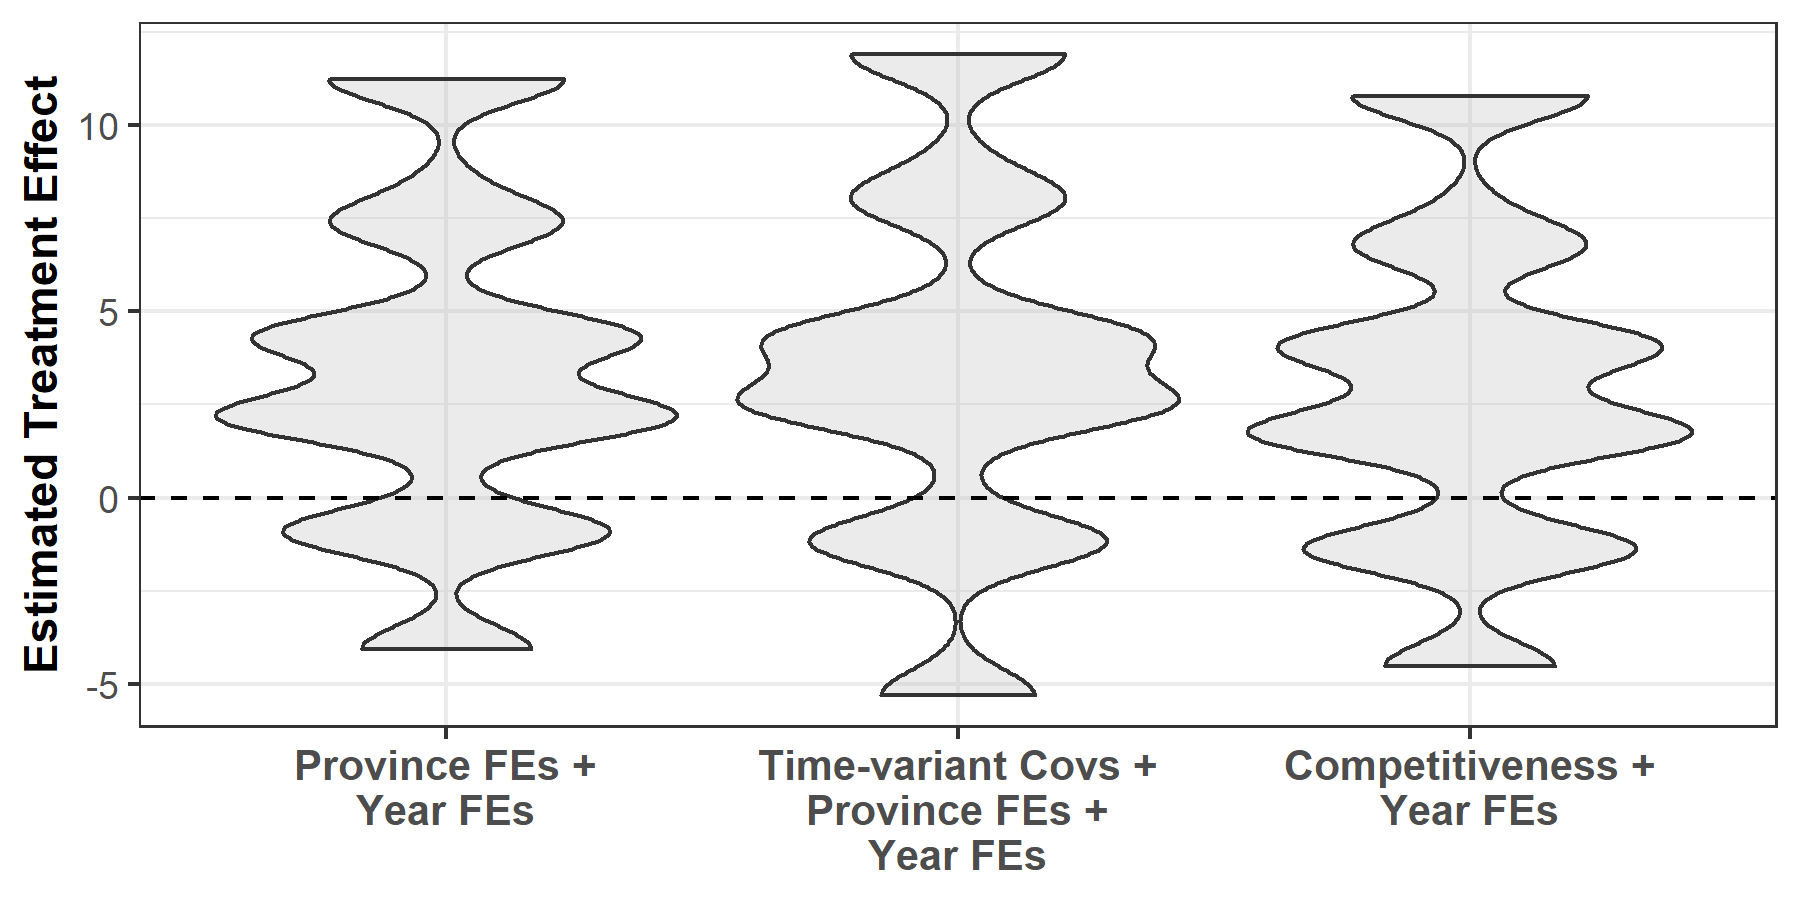
\includegraphics[width=.75\textwidth]{figure/200202_impute_results_2011.png}
	\captionsetup{singlelinecheck=off}
	\caption[Estimated linear fixed effects treatment effects using simulated vote shares]{Distribution of estimates of instantaneous treatment effects using linear fixed effects models on simulated samples. Each sample may include a different set of central candidate defeats and victories.}
	\label{fig:impute_results_2011}
\end{figure}

Distributions of estimated treatment effects using all the linear fixed effects models in the main analysis, obtained from $10000$ independent simulations of the vote shares, is shown in \autoref{fig:impute_results_2011}. It shows that the majority of the estimates are positive. Depending on specification, between .72 to .85 of the estimates are larger than zero. In other words, for the true estimate of localized defeats' treatment effects to be negative, the true vote shares of defeated candidates must have taken values that are highly improbable given the winning candidates' performance. Additionally, the negative estimates in \autoref{fig:lfe_placebo_2011} are close to the minimum values from the distributions, suggesting that almost any feasible allocations of defeated candidates' vote shares would lead to higher treatment effects. Altogether, although this evidence does not eliminate the possibility that the true treatment effect may be negative or close to zero, it does confirm that the linear fixed effects analysis using the entire sample of defeated central candidates is likely to be inaccurate. The generalized synthetic control method \citep{Xu2017gsynth}, on the other hand, not only addresses some concern about dynamic causality, but also produces estimates that seem much more probable. 

Overall, the positive effect from this analysis suggests that the CPV also reacted to localized defeats of its central candidates in the 2011 election by increasing central transfers to provinces that experienced such defeats. This finding, although much more tentative, is consistent with the result for the 2016 election.
 
\subsection{Responses to localized defeats in 2007 election}

The analysis for the 2007 election faces even more severe problems than the 2011 analysis. \autoref{fig:lfe_placebo_2007} shows estimates of the treatment effects, along with two sets of placebo treatment effects estimated for 2005 and 2006 (no placebo analysis is done for 2004 due to insufficient data). All these estimates are based on a sample with the entire set of central candidate defeats. The main treatment effects are estimated to be positive but not statistically significant, but the large and statistically significant (at .1 level, for some specifications) placebo treatment effects suggest that these estimates are likely to be inaccurate.

\begin{figure}[!htbp]
	\centering
	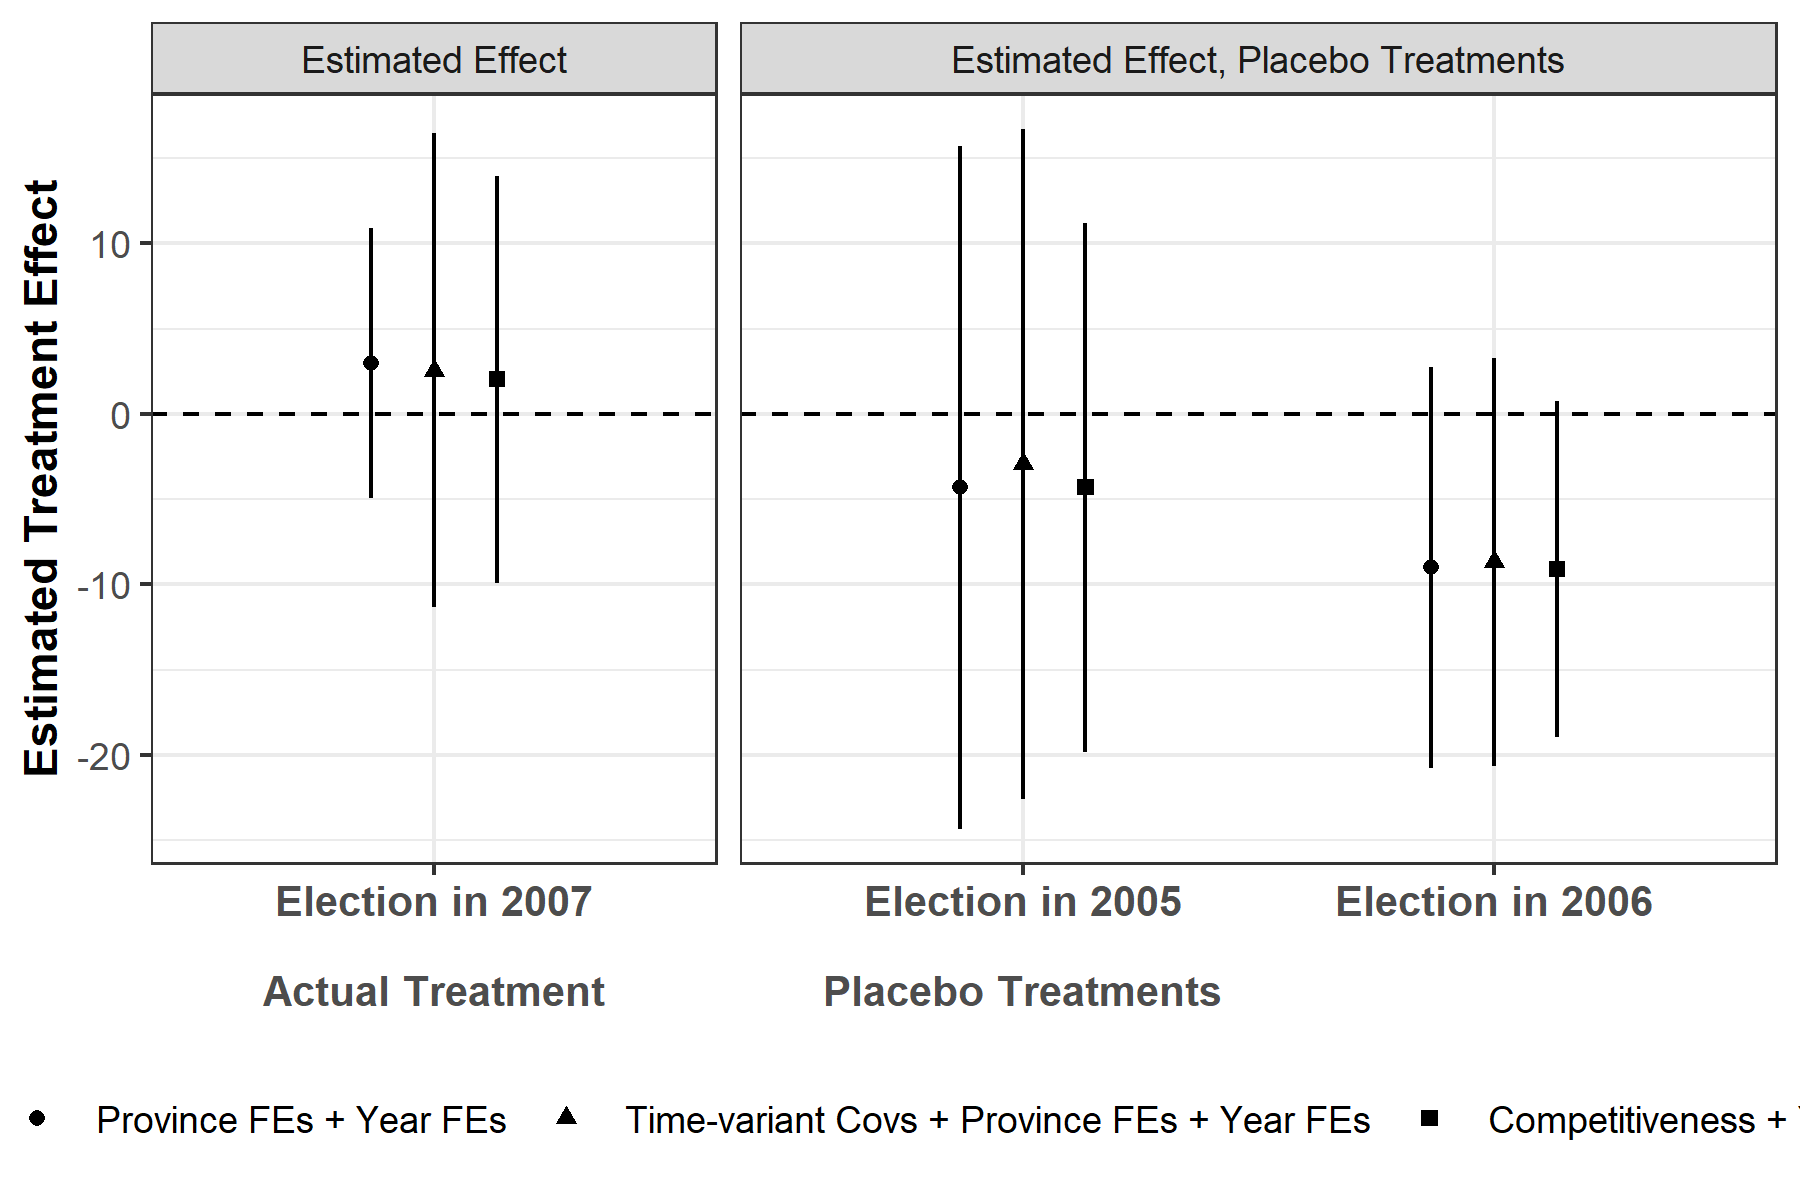
\includegraphics[width=.75\textwidth]{figure/200202_lfe_placebo_2007.png}
	\captionsetup{singlelinecheck=off}
	\caption[Estimated placebo linear fixed effects treatment effects]{Estimates of instantaneous treatment effects using linear fixed effects models. The error bars show 95\% confidence intervals.}
	\label{fig:lfe_placebo_2007}
\end{figure}

Unlike in the 2011 analysis, the generalized synthetic control method \citep{Xu2017gsynth} is not applicable for 2007 data because there are too few pre-treatment years to construct reliable synthetic controls. There is thus no reliable means to mitigate or eliminate the threat of dynamic causality evident in the large placebo effects. 

\begin{figure}[!htbp]
	\centering
	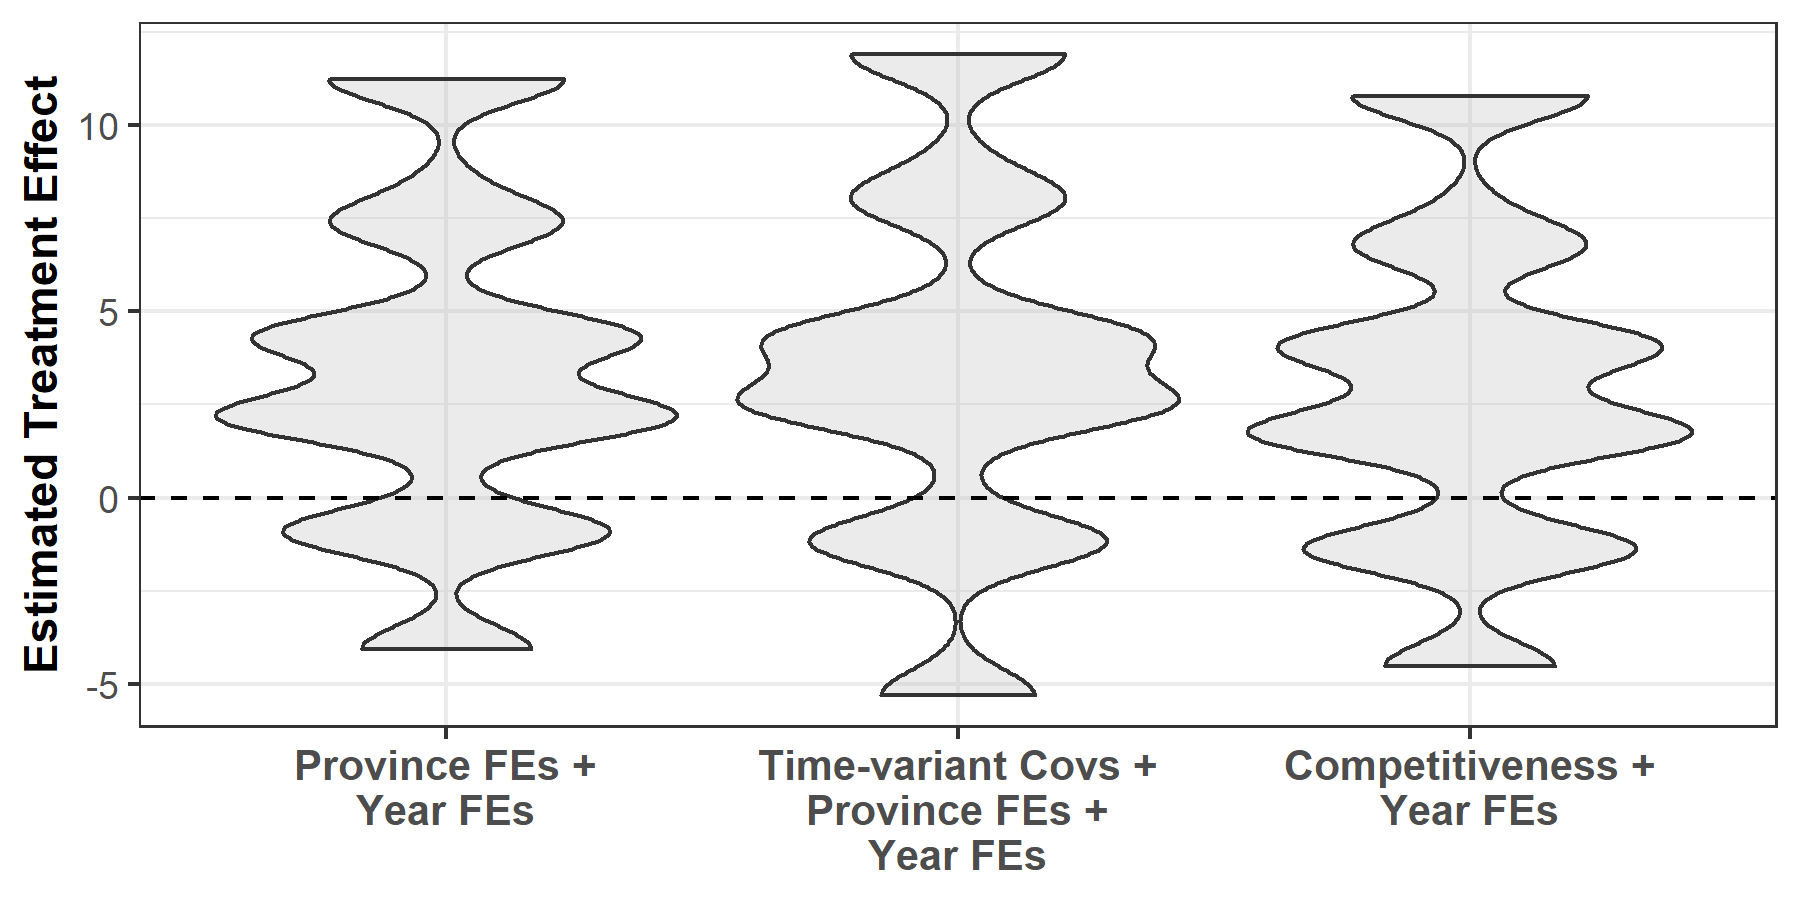
\includegraphics[width=.75\textwidth]{figure/200202_impute_results_2007.png}
	\captionsetup{singlelinecheck=off}
	\caption[Estimated linear fixed effects treatment effects using simulated vote shares]{Distribution of estimates of instantaneous treatment effects using linear fixed effects models on simulated samples.}
	\label{fig:impute_results_2007}
\end{figure}

At the same time, by simulating feasible vote shares of defeated candidates, I still find that the true estimates for the effect of localized defeats on central transfers, obtained when cases of heavy and unsurprising defeats have been excluded, are more likely to be positive. Specifically, \autoref{fig:impute_results_2007}, which shows the distribution of treatment effect estimates obtained from $10000$ simulations of vote shares for the defeatd candidates, confirms that the majority of feasible treatment effects are positive. Similar to the 2011 results, both the mean and median of the estimates are positive, with around .74 of the estimates found to be larger than zero. Even though much more data is needed for a stronger conclusion, this evidence does offer some reason to believe that the true treatment effects are larger than what found by the ``naive'' linear fixed effects models. Indeed, they are much more likely to be positive, which is consistent with the results for both the 2011 and 2016 elections.



\clearpage
\inputencoding{utf8}
\printbibliography[heading=bibintoc]


\end{document}


